\chapter{Návrh kvantového generátora náhodných bitov}

Táto kapitola sa zaoberá návrhom riešenia kvantového generátora náhodných čísel, ktorý využíva reálny kvantový hardvér a kvantovo korelované dvojice qubitov ako primárny zdroj náhodnosti.
Navrhnuté riešenie je implementované ako viacfázový proces, ktorý zahŕňa návrh kvantového zapojenia rešpektujúceho topológiu kvantového počítača, opakované merania kvantového obvodu, ako aj následný postprocesing nameraných dát a ich využitie pri generovaní náhodných čísel.

Dôraz je kladený na praktickú realizovateľnosť zapojenia na existujúcom kvantovom hardvéri, minimalizáciu systematického biasu a vytvorenie všeobecného modelu generácie, ktorý je prenositeľný aj na iné kvantové architektúry disponujúce fyzickými prepojeniami medzi qubitmi.

\section{Návrh kvantového zapojenia}

Základom navrhnutého kvantového generátora náhodných bitov je kvantové zapojenie, ktorého cieľom je efektívnym spôsobom využiť dostupné qubity kvantového počítača na generáciu náhodnosti.
Návrh zapojenia je zameraný predovšetkým na dve kľúčové požiadavky: maximalizáciu počtu využiteľných qubitov prostredníctvom tvorby kvantovo korelovaných dvojíc a rešpektovanie topológie kvantového počítača, ktorá určuje, ktoré qubity je možné priamo prepojiť pomocou dvojqubitových operácií.

Pri návrhu zapojenia je analyzovaná topológia použitého kvantového procesora s cieľom identifikovať maximálny počet dvojíc qubitov, ktoré sú prepojené jedným couplerom a umožňujú realizáciu CNOT brány.
Zvolený prístup zabezpečuje, že jednotlivé dvojice sú navzájom nezávislé a je možné ich paralelné spracovanie v rámci jedného kvantového obvodu.

V kontexte tejto práce sa pojmom \textit{kvantovo prepojená dvojica} rozumie dvojica qubitov, medzi ktorými bola vytvorená kvantová korelácia prostredníctvom dvojqubitovej operácie.
Takáto dvojica po meraní nevykazuje nezávislé správanie jednotlivých qubitov, ale produkuje korelované výsledky, ktoré sú využité na generáciu jedného náhodného bitu.

Meranie kvantového zapojenia je realizované jednorazovo pre všetky qubity v rovnakom časovom okamihu.
Každé takéto meranie predstavuje jeden \textit{shot} kvantového obvodu a vedie k získaniu binárneho vektora reprezentujúceho stav celého kvantového systému.

Schematické znázornenie základného kvantového zapojenia použitého pre jeden \textit{shot} kvantového obvodu je uvedené na obrázku~\ref{fig:quantumPair}.


\begin{figure}[H]
  \centering
  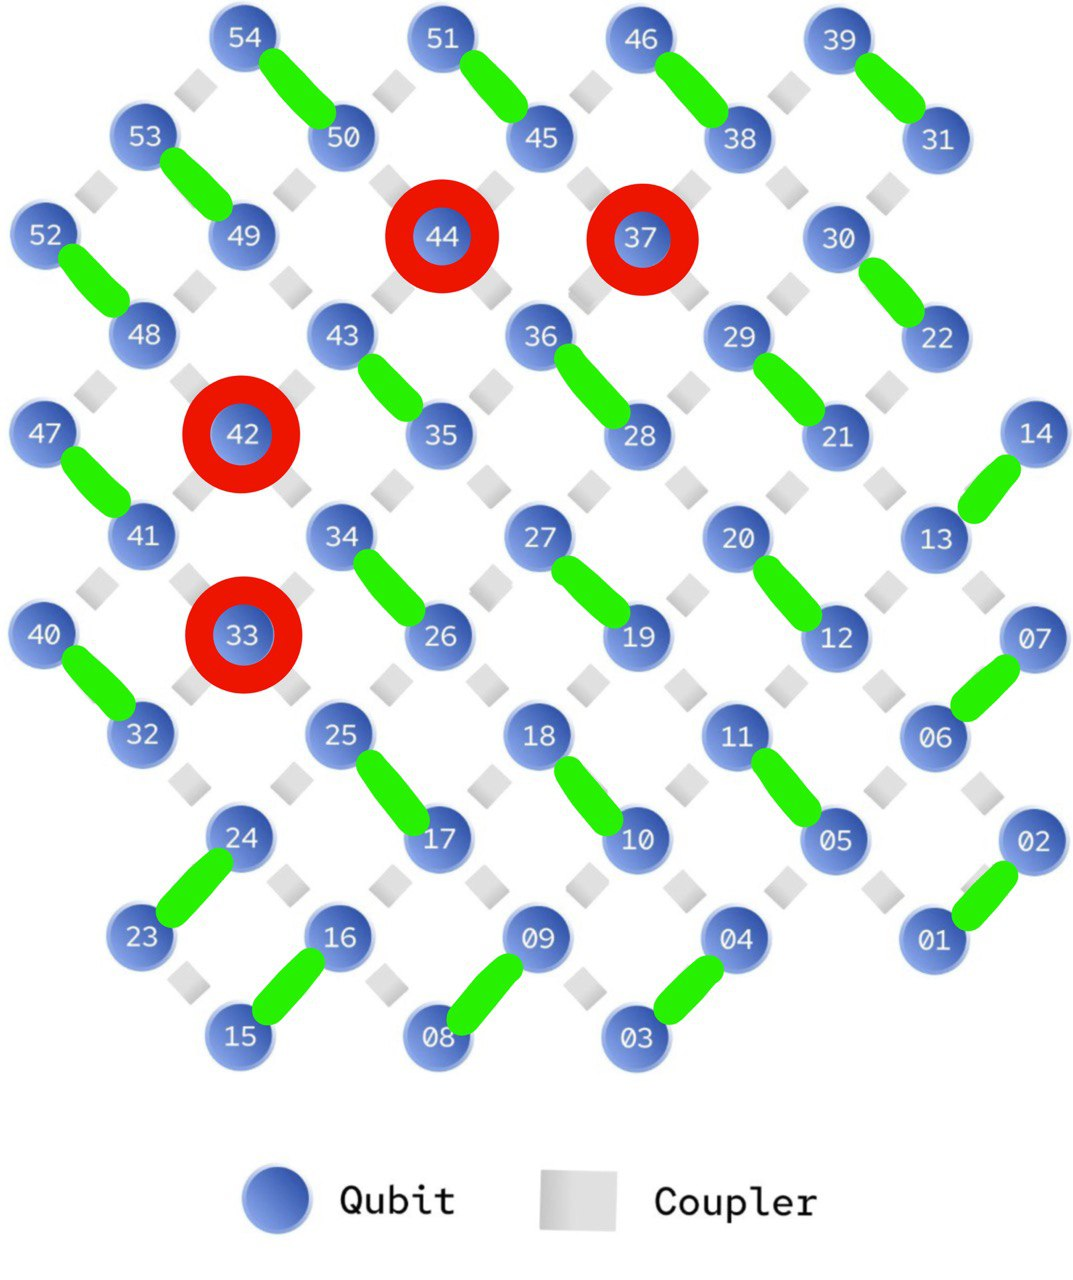
\includegraphics[width=0.6\textwidth]{images/QCzapojenie}
  \caption{Schematické znázornenie kvantového zapojenia, kde zelená farba reprezentuje kvantovo prepojené dvojice qubitov a červená farba označuje nevyužité qubity.}
  \label{fig:quantumPair}
\end{figure}

\subsection{Vytvorenie kvantovo korelovanej dvojice}

Každá kvantovo korelovaná dvojica v navrhnutom zapojení je vytvorená pomocou štandardného postupu založeného na aplikácii Hadamardovej a CNOT brány.
Prvý qubit dvojice je inicializovaný do základného stavu \(|0\rangle\) a následne je naň aplikovaná Hadamardova brána, ktorá qubit uvedie do rovnomernej superpozície stavov \(|0\rangle\) a \(|1\rangle\).

Následne je tento qubit použitý ako riadiaci qubit CNOT brány, pričom druhý qubit dvojice slúži ako cieľový qubit.
Podmienkou realizácie tejto operácie je existencia priameho fyzického prepojenia medzi qubitmi prostredníctvom jedného couplera, čo je zabezpečené výberom dvojíc na základe topológie kvantového procesora.

Výsledkom tejto sekvencie operácií je vznik kvantovo korelovaného stavu, ktorý po meraní nadobúda výlučne stavy \(|00\rangle\) alebo \(|11\rangle\).
Oba tieto výsledky nastávajú s rovnakou pravdepodobnosťou 50~\%, čo zabezpečuje rovnomerné rozdelenie generovaných hodnôt.
V kontexte generácie náhodných bitov je stav \(|00\rangle\) interpretovaný ako hodnota 0 a stav \(|11\rangle\) ako hodnota 1.

Použitím tohto prístupu je generácia náhodnosti založená na fyzikálnych vlastnostiach kvantového merania a nie na deterministickom algoritme.
Zároveň je minimalizovaný vplyv individuálneho biasu jednotlivých qubitov, keďže výsledný bit vzniká ako dôsledok interakcie dvoch qubitov a ich vzájomnej korelácie.


\subsection{Topologické limity kvantového zapojenia}

Hoci použitý kvantový počítač disponuje celkovo 54 qubitmi, nie je možné efektívne využiť všetky qubity na generáciu kvantovo korelovaných dvojíc.
Toto obmedzenie vyplýva z topológie kvantového procesora a dostupnosti fyzických prepojení medzi qubitmi.

Na základe analýzy topológie je možné vytvoriť maximálne 25 dvojíc qubitov, čo zodpovedá využitiu 50 qubitov.
Zvyšné qubity nie je možné zaradiť do dvojíc bez porušenia podmienky priameho prepojenia jedným couplerom.

Každé meranie kvantového zapojenia tak produkuje 25 náhodných bitov, ktoré sú následne spracované v ďalších fázach generácie.



%-----------------------------------------------------------------------------------------------------------------------------------------------------------

\section{Vplyv fyzikálnych vlastností kvantového hardvéru na generáciu náhodnosti}

Pri práci s reálnym kvantovým zariadením je nevyhnutné zohľadniť nielen abstraktný model kvantového výpočtu, ale aj praktické obmedzenia vyplývajúce z nedokonalostí fyzickej realizácie qubitov a kvantových operácií.

Osobitná pozornosť je venovaná javom ako decoherencia, chybovosť merania a individuálny bias qubitov, ktoré môžu ovplyvniť kvalitu generovaného bitového streamu.

\subsection{Charakteristiky kvantového hardvéru}

Parametre sú poskytované výrobcom kvantového zariadenia a predstavujú štatistické charakteristiky správania jednotlivých qubitov a kvantových brán.

Pre účely tejto práce boli analyzované najmä parametre súvisiace s časmi koherencie, presnosťou merania a fidelitou kvantových operácií.
Tabuľka~\ref{tab:qcSpecs} uvádza priemerné a mediánové hodnoty vybraných vlastností kvantového zariadenia použitého pri generácii náhodných bitov.

\begin{table}[H]
  \centering
  \caption{Vybrané technické charakteristiky kvantového hardvéru.}
  \label{tab:qcSpecs}
  \begin{tabular}{lcc}
    \hline
    \textbf{Vlastnosť} & \textbf{Priemer} & \textbf{Medián} \\
    \hline
    Čas relaxácie $T_1$ ($\mu$s) & 50.714 & 52.130 \\
    Čas dekoherencie $T_2$ ($\mu$s) & 14.641 & 14.446 \\
    Fidelita merania (\%) & 95.730 & 96.825 \\
    Fidelita simultánneho RB (\%) & 99.802 & 99.941 \\
    Fidelita CZ brány (\%) & 98.997 & 99.433 \\
    \hline
  \end{tabular}
\end{table}

Časy koherencie $T_1$ a $T_2$ určujú maximálne časové okno, v ktorom je možné vykonávať kvantové operácie bez výrazného vplyvu relaxačných a dekoherenčných javov, a nepriamo tak limitujú dĺžku a zložitosť realizovateľných kvantových zapojení.
Presnosť jednotlivých qubitov a kvantových operácií je však primárne charakterizovaná fidelitou merania, fidelitou jedno- a dvojqubitových brán a fidelitou simultánneho \textit{Randomized Benchmarking}.
Fidelita merania priamo vyjadruje pravdepodobnosť správnej identifikácie kvantového stavu pri jeho meraní, zatiaľ čo fidelita kvantových brán určuje mieru presnosti realizácie kvantových operácií.
Fidelita simultánneho RB poskytuje informáciu o správaní systému pri paralelnom vykonávaní operácií na viacerých qubitoch, čo je kľúčové pre návrh zapojení využívajúcich viacero kvantovo korelovaných dvojíc.
Tieto parametre majú priamy vplyv na spoľahlivosť výsledkov merania a kvalitu vytvárania kvantovo korelovaných dvojíc, a tým aj na výslednú kvalitu generovaného náhodného bitového streamu.

\subsection{Dopad decoherencie a biasu na návrh kvantového zapojenia}

Individuálne qubity použitého kvantového zariadenia vykazujú rozdielne úrovne decoherencie a mierne odlišný bias smerom k nameraným hodnotám 0 alebo 1.
Pri generácii náhodnosti založenej na meraní samostatných qubitov by tieto vlastnosti mohli viesť k systematickým odchýlkam v rozdelení výstupných bitov.

Navrhnuté riešenie preto využíva kvantovo korelované dvojice qubitov, pri ktorých výsledný bit vzniká ako dôsledok interakcie viacerých fyzikálnych procesov.
Do procesu generácie vstupujú individuálne vlastnosti oboch qubitov, kvalita fyzického prepojenia medzi nimi, presnosť realizácie dvojqubitových brán a časová stabilita kvantového zapojenia.

Kombinácia týchto faktorov vedie k zvýšenej komplexnosti systému, ktorá znemožňuje jednoznačne analyticky predpovedať výsledný bias smerom k hodnote 0 alebo 1.
Z pohľadu generácie náhodnosti je tento efekt žiadúci, keďže zvyšuje mieru nedeterministickosti výstupu.



%-----------------------------------------------------------------------------------------------------------------------------------------------------------



\subsection{Spracovanie zakázaných stavov}

Exportovaný súbor z výsledkov kvantového merania je následne manuálne nahraný na aplikačný server, kde prebieha ďalší postprocesing.
Na základe kľúča vytvoreného pri návrhu kvantového zapojenia sú rekonštruované pôvodné kvantovo korelované dvojice qubitov.
Každá rekonštruovaná dvojica je interpretovaná podľa nameraných hodnôt nasledovne:
stav \texttt{11} reprezentuje binárnu hodnotu 1 a stav \texttt{00} reprezentuje binárnu hodnotu 0.
Výskyty stavov \texttt{01} alebo \texttt{10} sú považované za zakázané stavy, ktoré vznikajú v dôsledku decoherencie alebo chýb kvantových operácií.

Pri spracovaní zakázaných stavov sú uvažované dva prístupy.
Tento rozdiel vyplýva z inherentnej povahy kvantových systémov, kde sa kvantové stavy môžu v dôsledku decoherencie alebo operácií nachádzať v medzistavoch, ktoré nie sú priamo interpretovateľné ako klasické bity 0 alebo 1.
Niektoré experimentálne prístupy preto tieto zakázané stavy úplne ignorujú, aby sa minimalizovalo riziko zavedenia chýb do výsledného bitového streamu.
Iné prístupy naopak tieto stavy mapujú na binárne hodnoty, čím sa zvyšuje počet použiteľných bitov a zároveň sa podporuje väčšia náhodnosť a homogenita generovaného streamu.
Tento rozdiel v spracovaní zakázaných stavov odráža kompromis medzi presnosťou interpretácie kvantových výsledkov a maximalizáciou kvality a náhodnosti výstupnej sekvencie.

\newpage
\paragraph{Zahrnutie bitov zo zakázaných stavov.}
V prvom prípade sú zakázané stavy mapované na binárne hodnoty, pričom stav \texttt{01} je interpretovaný ako 1 a stav \texttt{10} ako 0.
Grafické znázornenie tohto prístupu je zobrazené pre 25\,000-bitový stream, rozdelený do 10 rovnakých sekcií na overenie homogennosti a odchýlok od ideálneho stavu v tabuľke~\ref{tab:tableSoZakazanymi} a grafe~\ref{fig:biasNevynechaneChyboveStavy}.

\begin{table}[H]
  \centering
  \caption{Tabuľka bitov pri zahrnutí bitov zo zakázaných stavov}
  \begin{tabular}{c|c|c|c|c|c|c}
    Split & Celkom & Jednotky & Nuly & $p_0$ & $p_1$ & Bias \\
    \hline
    1 & 2500 & 1247 & 1253 & 0.50 & 0.50 & 0.00 \\
    2 & 2500 & 1285 & 1215 & 0.51 & 0.49 & 0.01 \\
    3 & 2500 & 1318 & 1182 & 0.53 & 0.47 & 0.03 \\
    4 & 2500 & 1318 & 1182 & 0.53 & 0.47 & 0.03 \\
    5 & 2500 & 1281 & 1219 & 0.51 & 0.49 & 0.01 \\
    6 & 2500 & 1337 & 1163 & 0.53 & 0.47 & 0.03 \\
    7 & 2500 & 1324 & 1176 & 0.53 & 0.47 & 0.03 \\
    8 & 2500 & 1287 & 1213 & 0.51 & 0.49 & 0.01 \\
    9 & 2500 & 1284 & 1216 & 0.51 & 0.49 & 0.01 \\
    10 & 2500 & 1231 & 1269 & 0.49 & 0.51 & 0.01 \\
    \hline
    \multicolumn{2}{c|}{Celkovo bitov} & \multicolumn{5}{c}{25\,000, Jednotky: 12\,912, Nuly: 12\,088, Bias=0.0164} \\
  \end{tabular}\label{tab:tableSoZakazanymi}
\end{table}

\begin{figure}[H]
  \centering
  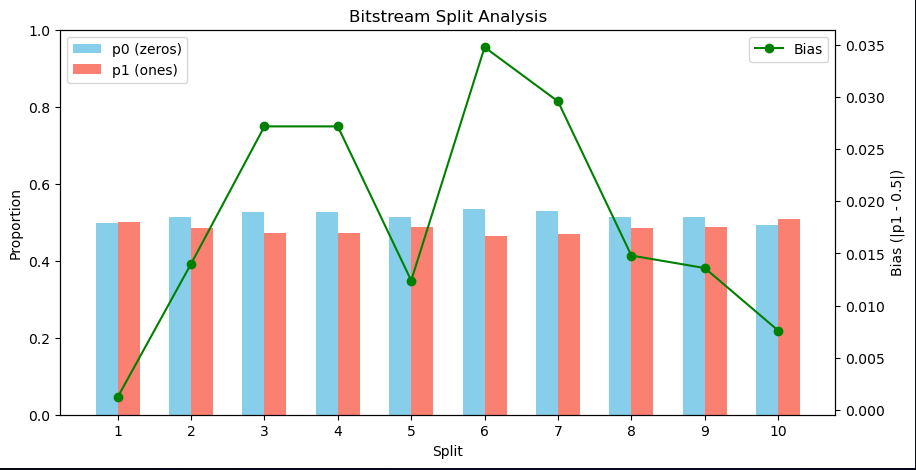
\includegraphics[width=0.9\textwidth]{images/biasNevynechaneChyboveStavy}
  \caption{Porovnanie biasu pri zahrnutí bitov zo zakázaných stavov a pri ignorovaní zakázaných bitov.}\label{fig:biasNevynechaneChyboveStavy}
\end{figure}

\newpage
\paragraph{Ignorovanie bitov zo zakázaných stavov.}
V druhom prípade sú zakázané stavy úplne vynechané a nie sú zahrnuté do výsledného bitového streamu.
Grafické znázornenie tohto prístupu je zobrazené pre 22\,239-bitový stream, opäť rozdelený do 10 sekcií na overenie homogennosti a odchýlok, ako ukazuje tabuľka~\ref{tab:tableBezZakazanych} a graf~\ref{fig:biasVynechaneChyboveStavy}.

\begin{table}[H]
  \centering
  \caption{Tabuľka bitov pri ignorovaní bitov zo zakázaných stavov}
  \begin{tabular}{c|c|c|c|c|c|c}
    Split & Celkom & Jednotky & Nuly & $p_0$ & $p_1$ & Bias \\
    \hline
    1 & 2223 & 1128 & 1095 & 0.51 & 0.49 & 0.01 \\
    2 & 2223 & 1153 & 1070 & 0.52 & 0.48 & 0.02 \\
    3 & 2223 & 1179 & 1044 & 0.53 & 0.47 & 0.03 \\
    4 & 2223 & 1202 & 1021 & 0.54 & 0.46 & 0.04 \\
    5 & 2223 & 1148 & 1075 & 0.52 & 0.48 & 0.02 \\
    6 & 2223 & 1207 & 1016 & 0.54 & 0.46 & 0.04 \\
    7 & 2223 & 1179 & 1044 & 0.53 & 0.47 & 0.03 \\
    8 & 2223 & 1169 & 1054 & 0.53 & 0.47 & 0.03 \\
    9 & 2223 & 1157 & 1066 & 0.52 & 0.48 & 0.02 \\
    10 & 2232 & 1116 & 1116 & 0.50 & 0.50 & 0.00 \\
    \hline
    \multicolumn{2}{c|}{Celkovo bitov} & \multicolumn{5}{c}{22\,239, Jednotky: 11\,638, Nuly: 10\,601, Bias=0.0233} \\
  \end{tabular}\label{tab:tableBezZakazanych}
\end{table}

\begin{figure}[H]
  \centering
  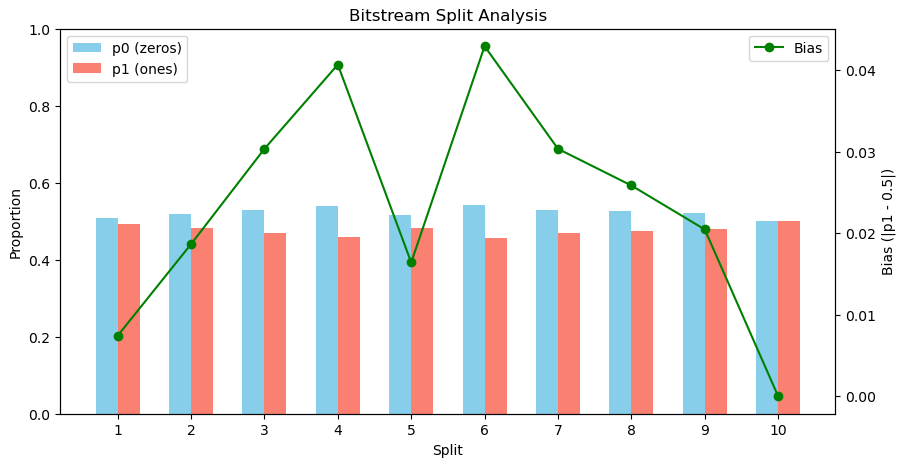
\includegraphics[width=0.9\textwidth]{images/biasVynechaneChyboveStavy}
  \caption{Porovnanie biasu bez zahrnutia bitov zo zakázaných stavov a pri ignorovaní zakázaných bitov.}\label{fig:biasVynechaneChyboveStavy}
\end{figure}

Zahrnutie bitov zo zakázaných stavov má pozitívny vplyv na kvalitu generovanej náhodnej sekvencie.
Hoci sa intuitívne môže zdať, že zakázané stavy predstavujú chybu, ich zaradenie do bitového streamu zvyšuje náhodnosť no ako je vidno v tab.\ref{tab:tableSoZakazanymi} nevyrovnáva homogénnosť.
Konkrétne, pri zahrnutí zakázaných bitov je celkový bias $0.0164$, zatiaľ čo pri ich ignorovaní je bias $0.0233$, čo je takmer dvojnásobný rozdiel.
Celkové rozdelenie bitov 0 a 1 je zároveň vyrovnanejšie no neexistuje žiadny rozdiel v homogénnosti streamu – všetky sekcie sú rovnomerne rozdelené bez ohľadu na to, či sú zakázané stavy zahrnuté alebo nie.
Tento fakt dokazuje, že použitie aj bitov zo zakázaných stavov je vhodné pre generovanie kvalitnej kvantovej náhodnosti bez negatívneho dopadu na rovnomernosť rozdelenia.





%-----------------------------------------------------------------------------------------------------------------------------------------------------------
\section{Ukladanie generovaných bitov do databázy}

Výsledné binárne hodnoty sú ukladané do databázy vo forme fixných blokov.
Každý databázový záznam obsahuje bitový reťazec s dĺžkou 25 bitov, pričom celkovo vzniká 1000 takýchto záznamov, zodpovedajúcich počtu vykonaných shotov kvantového zapojenia.

Jednotlivé databázové záznamy sú označené stavom použitia, pričom rozlišujeme záznamy, ktoré ešte neboli použité pri generácii náhodných čísel, a záznamy, ktoré už boli spotrebované.
Tento prístup umožňuje presnú evidenciu spotrebovanej kvantovej náhodnosti a zamedzuje opakovanému použitiu rovnakých bitov.
Taktiež je finančne efektívny a rýchly oproti alternatívam.

%-----------------------------------------------------------------------------------------------------------------------------------------------------------
\section{Tvorba náhodných bitových sekvencií}

Generácia náhodných čísel z uloženého bitového úložiska prebieha na základe výpočtu minimálneho počtu bitov potrebných na reprezentáciu požadovaného intervalu hodnôt.
Počet potrebných bitov je určený pomocou logaritmickej funkcie, ktorá zabezpečuje pokrytie celého rozsahu generovaných hodnôt.

Systém následne vyhľadá najbližší dostupný databázový záznam, ktorý obsahuje dostatočný počet nepoužitých bitov.
Tieto bity sú interpretované ako binárne číslo, ktoré je následne mapované na požadovaný interval.

Ako príklad možno uviesť generáciu náhodného čísla v rozsahu od 0 do 6.
V tomto prípade sú potrebné 4 bity, ktoré umožňujú reprezentovať hodnoty od 0 do 15.
Ak vzniknutá hodnota spadá mimo požadovaného intervalu, konkrétne nad hodnotu 6, príslušné bity sú označené ako tzv. spálené a nie sú ďalej použité.
Proces sa opakuje až do momentu, kým nie je získaná hodnota v požadovanom intervale, čím sa eliminuje systematický bias.

%-----------------------------------------------------------------------------------------------------------------------------------------------------------
\section{Algoritmický návrh kvantového generátora náhodnosti}

V sumarizácii bol vytvorený proces generácie kvantovej náhodnosti vo forme všeobecného modelu.
Navrhnutý model je koncipovaný tak, aby bol aplikovateľný na ľubovoľný kvantový systém s podporou dvojqubitových operácií a fyzických prepojení medzi qubitmi.
Proces je prezentovaný abstraktne a bez závislosti od konkrétnej implementácie, avšak bez ďalšieho experimentálneho overenia nie je možné jednoznačne tvrdiť, že je úplne nezávislý od konkrétneho kvantového zariadenia.

Všeobecný proces generácie kvantových náhodných čísel je možné zhrnúť do nasledujúcich krokov:

\begin{enumerate}
  \item Analýza topológie kvantového systému, ktorú je možné modelovať ako neorientovaný graf
  \begin{equation}
    G = (V, E),\label{eq:equation11}
  \end{equation}
  kde množina vrcholov $V$ reprezentuje qubity a množina hrán $E$ reprezentuje fyzické prepojenia (couplery) umožňujúce realizáciu dvojqubitových operácií.

  \item Výber maximálnej množiny disjunktných hrán
  \begin{equation}
    E' \subseteq E,\label{eq:equation10}
  \end{equation}
  pričom žiadne dve hrany nezdieľajú spoločný vrchol, s cieľom zabezpečiť paralelnú realizáciu kvantového zapojenia a minimalizáciu vzájomnej interferencie medzi qubitmi.


  \item Aplikácia Hadamardovej brány $H$ na prvý qubit každej vybranej dvojice, čím sa vytvorí rovnomerná superpozícia stavov
  \begin{equation}
    H \lvert 0 \rangle = \frac{1}{\sqrt{2}} \left( \lvert 0 \rangle + \lvert 1 \rangle \right).\label{eq:equation8}
  \end{equation}

  \item Vytvorenie kvantovej korelácie aplikáciou riadenej NOT operácie (CNOT) na každú dvojicu qubitov,
  kde riadiaci qubit je qubit nachádzajúci sa v superpozícii vytvorenej Hadamardovou bránou a cieľový qubit je druhý qubit dvojice.
  Touto operáciou vzniká korelovaný kvantový stav
  \begin{equation}
    \lvert \psi \rangle = \frac{1}{\sqrt{2}} \left( \lvert 00 \rangle + \lvert 11 \rangle \right),\label{eq:equation7}
  \end{equation}
  ktorý vykazuje maximálnu koreláciu výsledkov merania.

  \item Realizácia celkového merania kvantového registra na celom systéme, ktoré mapuje kvantový stav $\lvert \psi \rangle$ na binárny vektor
  \begin{equation}
    x \in \{0,1\}^{m},\label{eq:equation6}
  \end{equation}
  kde $m$ predstavuje počet meraných qubitov.

  \item Opakovanie merania kvantového zapojenia $N$-krát, čím vzniká množina realizácií
  \begin{equation}
    \mathcal{S} = \{ x_1, x_2, \dots, x_N \},\label{eq:equation5}
  \end{equation}
  ktorá tvorí surový bitový stream.

  \item Postprocesing nameraných dát zahŕňajúci rekonštrukciu pôvodných kvantových dvojíc a deterministické mapovanie korelovaných výsledkov merania na binárne hodnoty prostredníctvom mapovacej funkcie
  \begin{equation}
    f(\lvert 00 \rangle) = 0, \qquad
    f(\lvert 11 \rangle) = 1.\label{eq:equation4}
  \end{equation}

  \item Ukladanie výsledných bitov do perzistentného úložiska spolu s metadátami popisujúcimi ich stav použitia a pôvod.

  \item Generácia náhodných čísel je realizovaná výberom konečného počtu po sebe idúcich bitov z bitového úložiska a ich interpretáciou ako prirodzeného čísla.
  Pre požadovaný interval hodnôt $\langle 0, M \rangle$ je minimálny potrebný počet bitov $k$ určený vzťahom
  \begin{equation}
    k = \left\lceil \log_2(M + 1) \right\rceil.\label{eq:equation3}
  \end{equation}

  Zvolených $k$ bitov je interpretovaných ako binárne číslo
  \begin{equation}
    x = \sum_{i=0}^{k-1} b_i \cdot 2^i,\label{eq:equation}
  \end{equation}
  kde $b_i$ predstavujú jednotlivé bity získané z databázového úložiska.

  Ak výsledná hodnota $x$ nespĺňa podmienku
  \begin{equation}
    x \leq M,\label{eq:equation2}
  \end{equation}
  je tento výsledok zamietnutý a príslušné bity sú označené ako použité.
  Proces výberu ďalších bitov je opakovaný až do získania hodnoty spadajúcej do požadovaného intervalu.
\end{enumerate}


